\documentclass[11pt,letterpaper,english]{article}
\usepackage[T1]{fontenc} % Standard package for selecting font encodings
\usepackage{txfonts} % makes spacing between characters space correctly
\usepackage{xcolor} % Driver-independent color extensions for LaTeX and pdfLaTeX.
\usepackage{hyperref}  %The ability to create hyperlinks within the document
%\usepackage{blindtext} % To create text
%\usepackage{mdwlist} % mdwlist for compact enumeration/list items
%\usepackage[pagestyles]{titlesec} % related with sections—namely titles, headers and contents
\usepackage{fancyhdr} % header footer placement

\usepackage[top=1in, bottom=1in, left=1in, right=1in] {geometry} % Margins
\usepackage{graphicx}   % Essential for adding images to you document.

\usepackage{sectsty}
\sectionfont{\normalsize}
\subsectionfont{\normalsize}
\subsubsectionfont{\normalsize \it}

\usepackage[font=bf]{caption}
\captionsetup{labelsep=period}

\setlength{\parskip}{\baselineskip}%
\setlength{\parindent}{0pt}%


\pagestyle{fancy} % allows you to use the header and footer commands


\raggedright
\begin{document}

\setlength{\parindent}{0in} % Amount of indentation at the first line of a paragraph.

\pagestyle{fancy} \lhead{Title} \rhead{Lead PI} \renewcommand{%
\headrulewidth}{0.0pt}

\begin{center}
{\bf PROJECT NARRATIVE (The narrative should not exceed 15 pages)} 
\end{center}

\vspace{-.15in}

%\colorbox{yellow} {\bf {\emph{[Refer to the guidelines for additional instructions for preparing the proposal.]}}}

%\vspace{.15in}

{\bf References and visual materials, such as charts, graphs, pictures, etc., are included in the 15 page limit.} References should be included at the end of the Project Narrative. URLs that provide information related to the proposal should not be included  {\bf The 15-page limit will be strictly enforced.}  The Project Narrative should address the following points:

\vspace{-.25in}
\section{SIGNIFICANCE OF RESEARCH}
\vspace{-.2in}
List any previous INCITE award(s) received and discuss the relationship to the work proposed. Explain what advances you expect to be enabled by an INCITE award that justifies an allocation of petascale resources (e.g., anticipated impact on community paradigms, valuable insights into or solving a long-standing challenge, etc.). Place the proposed research in the context of competing work in your discipline or business. The information should be sufficient for peer review in your area of research and also appropriate for general scientific review comparing your proposal with proposals in other disciplines. Potential impact is the predominant determinant for awards. This factor will be assessed by a peer-review panel. Also list any previous INCITE award(s) received and discuss the relationship to the work proposed. {\bf This section is typically about 4 pages.}

When you cite a reference, please insert a number in brackets, as shown here [1], to correspond to its number on the reference list at the end of this template. Please call out the references in numerical order and list them in the same way. The reference list will count toward the 15-page limit.

Insert paragraph(s).
\vspace{-.25in}
\subsection{Heading 2 (optional)}
\vspace{-.2in}

Insert paragraph(s).

\vspace{-.25in}
\subsubsection{Heading 3 (optional)}
\vspace{-.2in}

Insert paragraph(s).

\vspace{-.25in}
\section{RESEARCH OBJECTIVES AND MILESTONES }  
\vspace{-.2in}
Describe the proposed research, including its goals and milestones and the theoretical and computational methods it employs. Goals and milestones should articulate simulation and developmental objectives and be sufficiently detailed to assess the progress of the project for each year of any allocation granted. Milestones should correlate with those in the milestone table. It is especially important that you provide clear connections between the project's overarching milestones, the planned production simulations, and the compute time expected to be required for these simulations (e.g., should correlate with those in the ``Use of Resources Requested''). {\bf This section is typically about 6 pages.}

If included, call out equations, tables, figures, and references in numerical order in text, such as Eqs. (\ref{Eq. 1}) and (\ref{Eq. 2}), Table \ref{Tab1}, and Fig. \ref{Fig1} below.

\vspace{-.15in}
\begin{equation} \label{Eq. 1} 
\partial ,\phi +u\cdot \nabla \phi =\nabla ^{2} \phi +\frac{1}{\tau } R\left(\phi \right)\, \, ,
\end{equation} 

\vspace{-.15in}
\begin{equation} \label{Eq. 2} 
\frac{\partial \phi }{\nabla \phi } =\frac{1}{2} \nabla ^{2} \phi \frac{e^{\frac{-R-R^{2} }{2u} } }{\left(2\tau \right)^{3N/2} } \sqrt{xyz} \, \, \sum 1+23\, \, \, . 
\end{equation} 

\begin{table}[h]
\centering
\caption{Table title}
\vspace{-.15in}
\label{Tab1}
\begin{tabular}{llll} \\ \hline 
\textbf{Column one} & \textbf{Column two} & \textbf{Column three} & \textbf{Column four} \\ \hline 
 xxx & xxx\textit{${}^{a}$} & xxx & xxx \\ \hline 
xxx & xxx & xxx & xxx \\ \hline 
{\textit{$^{a}$}Footnote here.} \\
\end{tabular}
\end{table}


\begin{figure}[h]
\centering
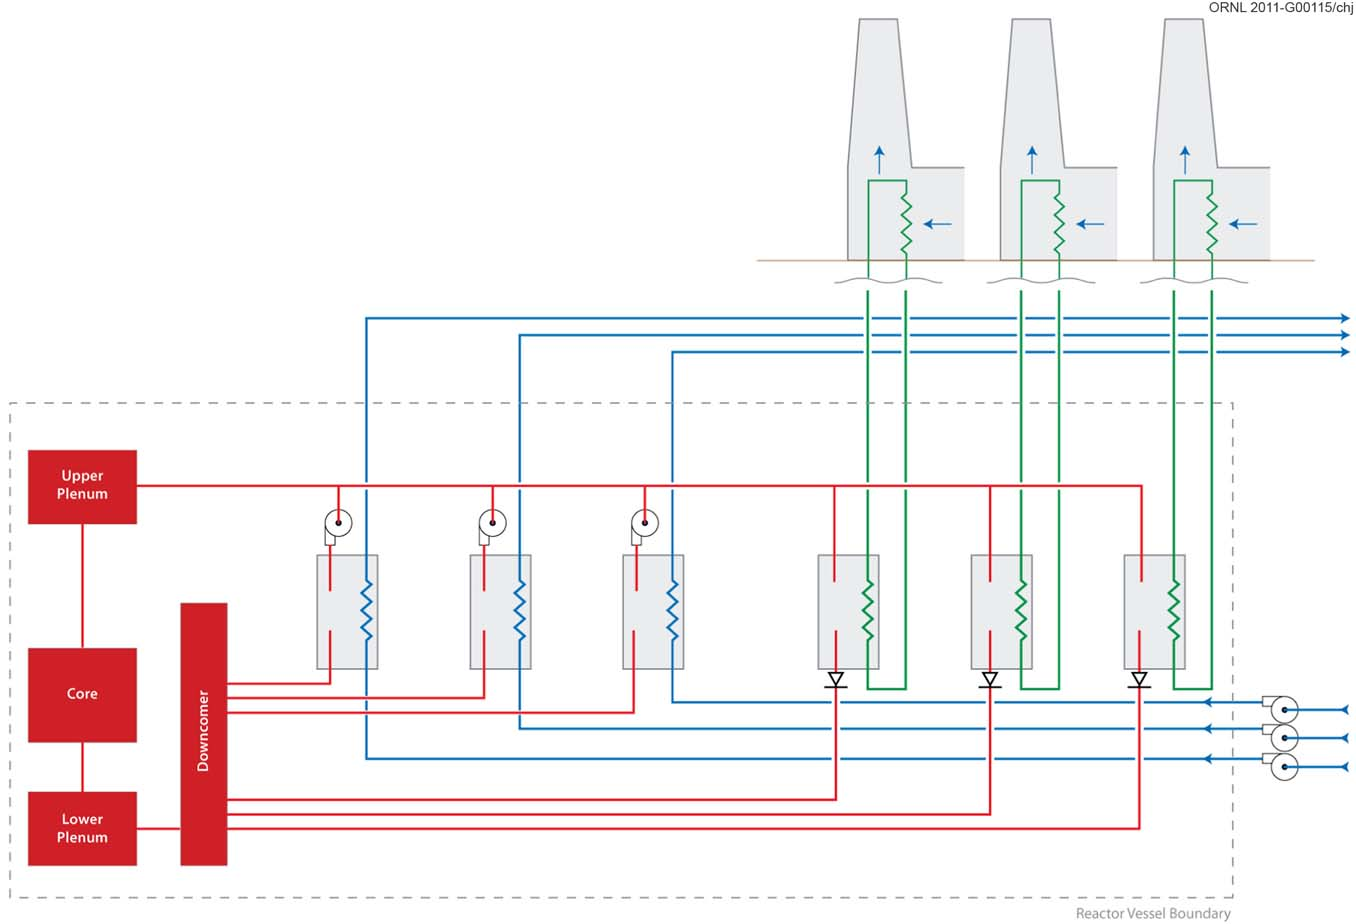
\includegraphics[width=4.52in, height=3.08in, keepaspectratio=true]{image1.jpg}
\caption{Figure caption.}
\label{Fig1}
\end{figure}

\vspace{-.25in}
\subsection{Heading 2 (optional)}
\vspace{-.2in}

Insert paragraph(s).

\vspace{-.25in}
\subsubsection{Heading 3 (optional)}
\vspace{-.2in}

Insert paragraph(s).

\vspace{-.25in}
\section{COMPUTATIONAL READINESS}
\vspace{-.2in}

Proposals will be assessed on the need for, readiness to use, and reasonableness of the request for resources. {\bf This section is typically about 5 pages.}

Insert paragraph(s).

\vspace{-.25in}
\subsection{Use of Resources Requested}
\vspace{-.2in}

Describe your proposed production simulations and state how the runs are tied to each of your project's goals and milestones (Section 4, "Milestone Table"). For the simulations you plan to carry out during production runs, provide a
\begin{enumerate}
\item description of what jobs are going to be run and how they relate to the research/development objectives given above;
\item description of processor/core use for large runs (e.g., 10,000-hour run with 100 cores, or ten 10-hour runs with 10,000 cores, for a 1,000,000-hour allocation); 
\item clear, detailed explanation as to how you calculated the requested number of processor hours; and 
\item summary of your anticipated annual burn rate (e.g., linear or with periods of peak usage).\\
\vspace{.1in}
In addition, describe the data storage requirements required by your production simulations.  If at any point during your project the sum of your data storage needs in the scratch filesystems exceed 1 petabyte, specific justification is required. For your production simulations, provide a:

\item Description of any input data set required, its size, and how you anticipate transferring it to the LCF.
\item Estimate and breakdown of the anticipated cumulative size of stored data, in scratch and long-term archival storage, at the end of the requested award. 
\item What is the effective lifetime of your useful data?  If the lifetime varies, show the breakdown by the total size used.  Explain the reason for the lifetime. 
\item What types of tools for data storage, compression (reduction), movement, and analysis do you currently use? Are the tools and/or applications needed ready or are there new capabilities or features you are developing?
\item If intending to make any fraction of the data generated public, please specify:
\begin{enumerate}
\item How much data and the scientific purpose
\item What tool will be used to share the data
\item From where will the data be shared\\
\vspace{.1in}
NOTE: The LCF data management policies can be found at

OLCF:  {\href{https://www.olcf.ornl.gov/computing-resources/data-management/data-management-user-guide/}{https://www.olcf.ornl.gov/computing-resources/data-management/data-management-user-guide/}}

ALCF:  {\href{http://www.alcf.anl.gov/user-guides/data-policy}{http://www.alcf.anl.gov/user-guides/data-policy}}
\end{enumerate}
\end{enumerate}

\vspace{-.25in}
\subsection{Leadership Classification}
\vspace{-.2in}

Summarize the requirement that best exemplifies the proposed computational work. Leadership targets in the INCITE program typically include one or both of the following categories: 

\vspace{-.25in}
\begin{enumerate}
\item Use of 20 percent or more of the system for production simulations. Parameter sweeps, ensembles, design of experiments, and other statistical methods that require large numbers of discrete or loosely coupled simulations may be considered capability-class campaigns. See the FAQS for details and qualifiers.
\item Specific architectural needs that can only be met by the LCF.
\end{enumerate}
\vspace{-.2in}
Insert paragraph(s).

\vspace{-.25in}
\subsection{Parallel Performance}
\vspace{-.2in}

Provide direct evidence, {\bf including supporting quantitative data}, for your production application's parallel performance for the intended research simulations. Ideally, the proposing team will have generated the data. If you cite work by others, explain why it is applicable here. You should use the application code you intend for the production work, not a related code. Data for sample systems not related to the intended research is undesirable. Performance benchmarking should reflect all I/O requirements. Parallel performance data in either strong or weak scaling mode must be provided. Explain how the strong or weak scaling applies to the proposed work. See the examples at the end of this document. 

NOTE: You may apply for a startup account at one of the centers to conduct performance studies. Applications are available at

ALCF: {\href{http://www.alcf.anl.gov/getting-started/apply-for-dd}{http://www.alcf.anl.gov/getting-started/apply-for-dd}}

OLCF: {\href{http://www.olcf.ornl.gov/support/getting-started/olcf-director-discretion-project-application}{http://www.olcf.ornl.gov/support/getting-started/olcf-director-discretion-project-application}}

\vspace{-.25in}
\subsection{Computational Approach}
\vspace{-.2in}

Provide a detailed description of your computational approach, including a discussion of the state of the art in the field. The description should also mention:

\vspace{-.25in}
\begin{enumerate}
\item Particular libraries required by the production and analysis software, algorithms and numerical techniques employed (e.g., finite element, iterative solver), programming languages, and other software used.
\item Parallel programming model(s) used (e.g., MPI, OpenMP/Pthreads and QPX intrinsics for BG/Q; MPI, OpenMP/Pthreads, CUDA, OpenACC or AVX intrinsics for XK7).
\item Project workflow including the role of analysis and visualization; identify where the analysis will be done and any potential bottlenecks in the analysis process.  Describe any analysis and/or data reduction tools used.
\item Software workflow solution (e.g., pre- and postprocessing scripts that automate run management and analysis) to facilitate this volume of work.
\item I/O requirements (e.g., amount, size, bandwidth, etc.) for restart, analysis, and workflow. Highlight any exceptional I/O needs.
\end{enumerate}

\vspace{-.25in}
\subsection{Developmental Work}
\vspace{-.2in}

For the computational approach above, describe what, if any, development work has been carried out to date, especially on the architecture of the requested resource. Describe what development work will be executed, and when,  during the proposed INCITE campaign.

\vspace{-.15in}
\section{REFERENCES}
\vspace{-.15in}

References are optional and may be structured in accordance with any style. They {\bf \em {do}} count toward the 15-page limit.
\vspace{-.15in}
\begin{enumerate}\itemsep0pt
\item First Author, Second Author, and Third Author, ``An article in a journal,'' {\em Journal Name} {\bf 32}(4): 46--52.\\
\item First Author and Second Author, {\em Report Title}, Report Number, Publishing Organization or Agency, City, State, 2013.
\item First Author et al., ``Chapter Title,'' {\em Book Title}, Publisher, City, State, 2011.
\item Corporate or Agency Author, {\em Book Title}, Publisher, City, State, 2012.
\end{enumerate}



\end{document}
